%%%%%%%%%%%
%\documentclass[10pt]{article}
\documentclass{llncs}
\pagestyle{plain}
\usepackage{color}
\usepackage{graphicx}
%\usepackage{a4wide}
%\usepackage{fullpage}
%\usepackage{epsfig}
\usepackage{amsfonts}
\usepackage{latexsym,amssymb,amsmath}
\usepackage{todonotes}
\usepackage[colorlinks=true, allcolors=blue]{hyperref}

%\usepackage{amsmath}
%\usepackage[T1]{fontenc}
%\usepackage{natbib}
%\usepackage{algorithmicx}
\usepackage[ruled]{algorithm}
\usepackage[noend]{algpseudocode}
\algdef{SE}[DOWHILE]{Do}{doWhile}{\algorithmicdo}[1]{\algorithmicwhile\ #1}
%\usepackage{algorithm}
%\usepackage{algpseudocode}
\usepackage{comment}
\usepackage{epstopdf}
\usepackage{epsfig}
%Example1: \epsfig{width=8cm,file=FIG/lb1.pdf}
%Example2: \epsfig{width=8cm,file=FIG/lb1.eps}
\usepackage{soul}

\setcounter{tocdepth}{3}
\setcounter{secnumdepth}{3}
%\usepackage[hidelinks]{hyperref}


%\usepackage[appendix=append]{apxproof}
%\renewcommand{\appendixprelim}{\section*{Appendix}}
%\renewcommand{\appendixsectionformat}[2]{Proofs From Section~#1\ (#2)}
%\renewcommand{\appendixprelim}{\clearpage\onecolumn\newpage\section*{Appendix}}


%\newtheorem{example}{Example}
%\newtheorem{definition}{Definition}
%\newtheorem{axiom}{Axiom}
%\newtheorem{lemma}{Lemma}
%\newtheorem{theorem}{Theorem}
%\newtheorem{corollary}{Corollary}
%\newtheorem{problem}{Problem}
%\newtheorem{remark}{Remark}
%\newenvironment{proof}{\noindent{\bf Proof.}}{\hfill \qed \vskip 5pt}
%\def\qed{\hfill\rule{2mm}{2mm}}
%\newcommand{\ep}{\qed}


\newcommand\JC[1]{{\color{blue} JC: #1}}         % Jared:    Use \JC{my note}


\begin{document}

\title{The Good Cop and the Oblivious Fugitive}

\author{
Evangelos Kranakis\inst{1}\inst{2}
%\and
%Danny Krizanc\inst{2}
}

\institute{
School of Computer Science, Carleton University, Ottawa, Ontario, Canada.
%\and
%Dep. of Math. \& Computer Science, Wesleyan University, Middletown CT, USA.
\and
Research supported in part by NSERC Discovery grant.
}
\maketitle

\centerline{\today}

\begin{abstract}
A fugitive has escaped from jail and is running away from it along a half-infinite street at constant speed $v <1$. The jail is placed at the origin of the infinite half-line $[0,+\infty)$. A policeman (modelled as an autonomous mobile agent) starting at a point (denoted by $s$) on this street wants to catch the fugitive and bring him back to jail. The policeman and the fugitive start at the same time but the policeman does not know the starting position (denoted by $d$) of the fugitive. 

We give search and delivery algorithms to solve the problem under two possible scenarios: 1) when $v$ is known and $d$ is unknown, and 2) when both $v$ and $d$ are unknown to the policeman. We prove that the corresponding competitive ratios with respect to an all powerful searcher that knows both $v$ and $d$ are $1+\frac{v + \sqrt{2-v^2}}{1-v}$ and $1 + \frac{2(1+v)}{1-v}$, respectively, and these are optimal.

\vspace{0.5cm}
\noindent
{\bf Key words and phrases.} Agent, Fugitive, Knowledge, Mobile, Oblivious, Policeman, Searcher.

\end{abstract}


%\newpage

%\section{Introduction}
%
%\hl{To do}
%We consider. 
%
%\subsection{Model}
%
%\subsection{Notation and Terminology}
%
%\subsection{Related work}
%
%\subsection{Outline and results of the paper}

%\begin{figure}[!htb]
%\begin{center}
%\includegraphics[width=10cm]{FIG/th1.pdf}
%\end{center}
%\caption{An arrangement of seats; moviegoers may enter only from the left
%and the numbering of the seats is $1$ to $n$ from left to right.}
%\label{fig:th1}
%\end{figure}

%\vspace{-0.3cm}
%\begin{algorithm}[H]
%\caption{Rectilinear Algorithm ($S$ source, $D$ destination)}\label{alg:rect1}
%\begin{algorithmic}[1]
%\State {Every robot $r$ moves vertically towards the line $SD$;} 
%\If {the $x$-coordinate of robot $r$ is outside the segment $SD$}
%\State{$r$ moves first towards $S$, exchanges information with the robots it meets along the way, and if it meets a robot which already has the message it changes direction and continues towards $D$;}
%\Else
%\If {if at the time of $r$'s arrival in the segment $SD$ there is no other robot to its right carrying the message towards $D$} 
%\State{it moves left towards $S$, exchanges information with the robots it meets along the way, and if it meets a robot which already has the message it changes direction and continues towards $D$;}
%\Else 
%\State{if at the time of $r$'s arrival in the segment $SD$ there is another robot to its right carrying the message towards $D$ then it moves right towards $D$;}
%\EndIf
%\EndIf
%\end{algorithmic}
%\end{algorithm}

\section{Introduction}

%\hl{Focus on variations of cops and robbers}
The ``cops and robbers'' problem were introduced by Nowakowski and Winkler in~\cite{nowakowski1983vertex} and Quilliot~\cite{quilliot1985short}, independently, cf., also Frieze et al.~\cite{frieze2012variations}. These are perfect information games with two players consisting of a set of cops and a robber which can move along the vertices of a graph. The cops and the robber occupy vertices of the graph in alternate rounds and the game ends if the cops and the robber are colocated on a vertex of the graph. For additional information on  search and robber problems, cf. Bonato~\cite{bonato2011game}.

We study a similar problem here whereby a good cop wants to catch an oblivious fugitive and bring him back to jail. The cop is ``good'' because it wants to employ the fairest and fastest algorithm, depending on its knowledge about the fugitive, while the fugitive is ``oblivious'' in that it moves away from the origin without ever changing its behaviour throughout the search process. The algorithm is executed in a continuous (as opposed to discrete) setting on the infinite half-line.

\subsection{Catching an Oblivious Fugitive}

A policeman (modelled as an autonomous mobile agent) and a fugitive are on the half-infinite line $[0, +\infty)$. The policeman starts at a point $s \geq 0$ and can move with speed $1$, while the fugitive at a point $d > 0$ and can move with constant speed $v<1$ away from the origin (see Fig.~\ref{fig:fugi0}). 
\begin{figure}[!htb]
\begin{center}
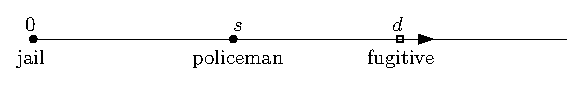
\epsfig{width=8cm,file=FIG/fugi0.eps}
\end{center}
\caption{Starting positions of the policeman at the point $s\geq 0$ and the fugitive at the point $d\geq 0$ on the infinite half line. The jail is at the origin. The fugitive is oblivious and is moving away from the jail at constant speed $v<1$.}
\label{fig:fugi0}
\end{figure}
The jail is located at the origin. The fugitive is oblivious and moves with constant speed. We are interested in solving the following problem.
\begin{problem}
Give an algorithm with optimal competitive ratio for the policeman to catch the fugitive and bring him to jail.
\end{problem}

\subsection{Model and Assumptions}

In the sequel the policeman will be called ``searcher'' because it must also search to find the fugitive. We call the half-open interval $[0, +\infty)$ ``half-line''. During the search the fugitive is oblivious in that it moves at constant speed $0 \leq v<1$  from the origin and never stops or changes direction of movement. The searcher can move anywhere on the infinite half-line, change direction, stop and restart, and ``carry'' the fugitive (when it catches him) without exceeding its max speed $1$; the speed of the searcher is not affected when carrying the fugitive. The searcher starts at a point $s\geq 0$ and the fugitive at a point $d>0$ on the half-line. The starting position $d$ is unknown to the searcher, moreover the searcher and the fugitive start at the same time. 

An instance $I$ of the search and delivery problem is determined by the starting locations of the cop $s$ and the fugitive $d$ and its speed $v<1$. $T_{opt} (I)$ is the optimal time it takes an omniscient cop who has full knowledge of the input $I$ in order to catch and bring the fugitive to jail; $T_A (I)$ is the time it takes the algorithm $A$ to perform the same task given its  (limited) knowledge.  We denote by 
$
CR_A = \sup_I \tfrac{T_A(I)}{T_{opt} (I)}
$ 
the worst-case competitive ratio of algorithm $A$ to deliver on any input $I$. Further, we denote the competitive ratio of search and delivery by
$
CR = \inf_{A} CR_{A},
$
where the infimum is taken over all possible delivery algorithms $A$ on the circle which deliver successfully the object.

%\subsection{When $d$ is Known to the Searcher}


\subsection{Related Work}

Competitive algorithms for search have been considered in numerous scientific studies due to their importance for the analysis of algorithms in theoretical computer science. The seminal book by Alpern and Gal~\cite{alpern03} is a good source for studies on search games and rendezvous. Baeza-Yates et al.~\cite{baezayates1993searching} initiated and considered search problems by a single robot in an infinite line or in the plane. Our approach will not involve the doubling, but is worth mentioning Chrobak and Kenyon-Mathieu in~\cite{chrobak2006sigact} which give a survey of the “doubling” method which uses geometrically increasing estimates on the optimal solution to produce fragments of the desired solution in online and offline approximation algorithms. 

The concept of searching for moving target was initiated by McCabe~\cite{mccabe1974searching} in a stochastic setting on an infinite discrete line. Demaine et al.~\cite{demaine2006online} initiated search analysis when turning is counted as a cost. Bose et al.~\cite{bose2013revisiting,bose2017general} derive optimal competitive search strategies for a search problem variant where the target is moving and the searcher’s cost at each step is a constant times the length of the step plus a fixed constant turn cost. Bonato et al.~\cite{bonato2020probabilistically} study $p$-Faulty Search, whereby a probabilistically faulty robot searches the half-line for a hidden item. More recently, Coleman et al.~\cite{coleman2023line} consider and analyze knowledge competitive ratio tradeoffs in searching for a mobile target in an infinite line and Coleman et al. in~\cite{iwoca_journal_version} obtain optimal competitive ratio when the speed of the mobile is unknown. Additional work in more complex topologies can be found in Ortiz and Schuierer~\cite{lopez2001ultimate} for search on $m$-rays, and more generally in Koutsoupias et al.~\cite{koutsoupias1996searching} which combinatorial optimization problems related to searching a known graph, for a target located at an unknown node.  

Related to our present work there are also several recent studies on the search and delivery problem especially due to its applicability to automated robotic delivery of objects. Carvalho et al.~\cite{del_carvalho_graph} analyze the problem on graphs, and Coleman et al.\cite{coleman2024optimal} consider the problem of how to efficiently recover and complete the delivery of an object in the plane under the presence of a faulty robot. Closely related to our study is the recent work of Coleman et al.~\cite{coleman2023search} which analyzed the search and delivery problem considered in our present paper for a static target in both a finite segment and the infinite half-line.

\subsection{Results}


In the sequel we design algorithms for the cases when the starting position $d$ of the fugitive is either known or unknown to the searcher. In all cases we compare the ratio of the time it takes the algorithm to catch the fugitive divided by the time it takes an omniscient searcher (having full knowledge of the environment) to find the fugitive and deliver him to the origin.  


If $d$ is known to the searcher then it is simple to prove tight upper and lower bounds regardless of whether or not the speed of the fugitive is known.
We consider two cases.

{\bf Case 1: $d \leq s$.}\\
The algorithm for the searcher is 
\begin{equation}
\label{eq:algo1}
s \to 0.
\end{equation}
The searcher moves in the direction of the origin; it catches the fugitive and delivers him to the origin. 

{\bf Case 2: $s < d$.}\\
The algorithm for the searcher is 
\begin{equation}
\label{eq:algo2}
s \to +\infty \to 0.
\end{equation}
The searcher moves in the direction of the fugitive. It catches the fugitive at time $\frac{d-s}{1-v}$. At that time the adversary is in position $d+\frac{(d-s)v}{1-v}$. The total time is $\frac{d-s}{1-v} + d+\frac{(d-s)v}{1-v} = d + \frac{(d-s)(1+v)}{1-v}$.
 It is easy to see that both algorithms have optimal competitive ratio equal to $1$. 

Since the case when $d$ is known is trivial, in the sequel we consider only the case when $d$ is unknown to the searcher. This includes the two cases when $v$ is known and when $v$ is unknown. Here is a summary of the results.
\begin{table}[htp]
\caption{Upper and lower bounds on the competitive ratio of search and delivery for various knowledge models; $v$ is the speed of the fugitive and $d$ is the distance of the fugitive at the start.}
\begin{center}
\begin{tabular}{| l | c | }
\hline
Knowledge & UB \& LB \\
\hline
\hline
$d$ Known & 1 \\
\hline
$d$ Unknown \& $v$ Known & $1+\frac{v + \sqrt{2-v^2}}{1-v}$ \\
\hline
$d$ Unknown \& $v$ Unknown & $1 + \frac{2(1+v)}{1-v}$ \\
\hline
\end{tabular}
\end{center}
\label{default}
\end{table}%

%The case when $d$ is known is easy and was discussed above. The main results are proved in the sequel. 
%It is also easy to check that 
%$$
%\frac{1 + \sqrt{2-v^2}}{1-v} < 1 + \frac{2(1+v)}{1-v},
%$$
%for all $v < 1$.

%There remains to close the gap between the upper and lower bounds on the competitive ratios for the case when $d$ is unknown and $v$ is known.

In the rest of the paper we consider the case when $d$ is unknown to the searcher. In Section~\ref{Speed $v$ is Known to the Searcher}  we consider the case when $v$ is known to the searcher, and in Section~\ref{Speed $v$ Is Unknown to the Searcher} the case when $v$ is unknown. In both instances we prove tight upper and lower bounds.


\section{Speed $v$ is Known to the Searcher}
\label{Speed $v$ is Known to the Searcher}

We prove upper and lower bounds.

\subsection{Upper Bound}

In the sequel we employ a parameter $x > s$ indicating a guess made by the searcher and consider the following algorithm abbreviated as
$$
s \to x \to 0 \to +\infty .
$$
The parameter $x$ used in the algorithm will be determined in the sequel. In more detail the algorithm is as follows.
\begin{enumerate}
\item The searcher follows path $s \to x;$ 
\item {\bf If} at any time during this traversal the searcher finds the fugitive, it brings him to the origin and stops;
\item {\bf Else} searcher upon reaching the point $x$ it returns to the origin by following the path $x \to 0$;
\item Upon reaching the origin, the searcher follows the path $0 \to +\infty$ and when it catches the fugitive it brings him to the origin;
\end{enumerate}

In the analysis of the algorithm we will show that the optimal choice for $x$ will be
$$
x = \frac{2-v + \sqrt{2-v^2}}{2(1-v)} \cdot s,
$$
which the searcher can employ because it knows the value of $v$.


\begin{theorem}[Upper Bound when Speed $v$ is Known]
\label{thm:CR-mobile}
The competitive ratio of the previous search and delivery algorithm for a mobile fugitive moving away from the origin with constant speed $v<1$ is
$$
%\frac{\frac{2-v \pm \sqrt{2-v^2}}{2(1-v)} \cdot s}s-1
%\frac{1 + \sqrt{2-v^2}}{1-v} 
1 + \frac{v + \sqrt{2-v^2}}{1-v}.
$$
\end{theorem}

\begin{proof} (Theorem~\ref{thm:CR-mobile})
Let $A$ denote the algorithm above and $T_A$ its cost. Also $T_{Opt}$ is the cost of the optimal offline algorithm.  
%\subsection{Analysis of the Algorithm}
We consider several cases depending on the relative sizes of the parameters $d, s, x$.

{\bf Case 1: $d < s$.} (see Fig.~\ref{fig:fugi1}.)\\
Since $d <s$ it is clear that $T_{opt} = s$. 
\begin{figure}[!htb]
\begin{center}
\epsfig{width=8cm,file=FIG/fugi1.eps}
\end{center}
\caption{$d < s$.}
\label{fig:fugi1}
\end{figure}
Since $x>s$, we have that $T_A = x-s + x = 2x -s$. It follows that
\begin{equation}
\label{eq:case1}
CR_1 = \frac{T_A}{T_{opt}} = \frac{2x-s}{s} = \frac{2x}s - 1.
\end{equation}

{\bf Case 2: $s \leq d \leq x$.}  (see Fig.~\ref{fig:fugi2}.)\\
The searcher will catch the fugitive in time $\frac{d-s}{1-v}$; 
\begin{figure}[!htb]
\begin{center}
\epsfig{width=8cm,file=FIG/fugi2.eps}
\end{center}
\caption{$s \leq d \leq x$.}
\label{fig:fugi2}
\end{figure}
since it started at $s$ it will now be located at the point $s+\frac{d-s}{1-v}$ so it will take the searcher additional time $s+\frac{d-s}{1-v}$ to reach the origin. Therefore $T_{opt} = s+ 2\frac{d-s}{1-v}$.

{\bf Case 2a. If $s + \frac{d-s}{1-v} \leq x$ then $CR_2 = 1$.} \\
The searcher starts at $s$ and the fugitive starts at $d$, where $s \leq d \leq x$. The searcher could reach the fugitive in time $\frac{d-s}{1-v}$. Since $s + \frac{d-s}{1-v} \leq x$ the searcher will in fact catch the fugitive before reaching $x$ and can therefore return him to the origin. As a consequence, $T_A = s+ 2\frac{d-s}{1-v} = T_{opt}$ and $CR_2 = 1$.

{\bf Case 2b. If $s + \frac{d-s}{1-v} > x$ then $CR_2$ is given in Equation~\eqref{eq:case2}.}\\
As before, the searcher starts at $s$ and the fugitive starts at $d$, where $s \leq d$. The searcher could reach the fugitive in time $\frac{d-s}{1-v}$ but since $s + \frac{d-s}{1-v} > x$ the searcher will not be able to travel far enough (since according to the algorithm it would have to stop and change direction at $x$) and will therefore miss the fugitive in its first. So it will return to the origin and follow the trajectory $0 \to +\infty$ until it catches the fugitive and return him to the origin. When the searcher returns to the origin for the first time, total time 
$$
T_0 = 2x-s
$$ 
has already passed and the fugitive will be in position 
$$
d+ ((x-s)+x) v = d + (2x-s)v. % \left(s+ 2\frac{d-s}{1-v}\right)v
$$
when the searcher is at the origin. 
The searcher will now follow the path $0 \to +\infty$ and will catch the fugitive in additional time 
$$
T_1 = \frac{d + (2x-s)v}{1-v} 
$$
and return him to the origin in further additional time $T_1$. Therefore algorithm $A$ takes total time 
$$
T_A = T_0 + 2 T_1 = 2x-s + 2\frac{d + (2x-s)v}{1-v} .
%x-s + 2 \frac{d+\left(s+ 2\frac{d-s}{1-v}\right)v}{1-v} 
$$
The competitive ratio as a function of $x$ will be
\begin{equation}
\label{eq:case2}
CR_2 (d) = \frac{T_A}{T_{opt}} = \frac{2x-s + 2\frac{d + (2x-s)v}{1-v} }{s+ 2\frac{d-s}{1-v}}  .
\end{equation} 
Equation~\eqref{eq:case2} is valid as long as the condition $s+\frac{d-s}{1-v} > x$,
which is equivalent to $d > s + (x-s)(1-v)$.

The resulting competitive ratio will be
\begin{align}
CR_2 
&= \notag \sup_{s \leq d \leq x} CR_2 (d) \\
&= \notag 
\sup_{s \leq d \leq x} \frac{2x-s + 2\frac{d + (2x-s)v}{1-v} }{s+ 2\frac{d-s}{1-v}}  \\
&= \notag
\sup_{s \leq d \leq x} \left(1+\frac{2x(1+v)}{2d -s (1+v)}\right) \\
&= \notag
1+\frac{2x(1+v)}{2 (s + (x-s)(1-v)) -s(1+v)}\\
&= \label{eq:case2a} 
1+\frac{2x(1+v)}{(1-v)(2x-s)}
\end{align} 
%Note that for $v=0$, $CR_2 = \frac{x-s + 2 \frac{d+\left(s+ 2\frac{d-s}{1-v}\right)v}{1-v}}{s+ 2\frac{d-s}{1-v}} = \frac{x-s+2d}{s+2(d-s)}$

{\bf Case 3: $x < d$.}  (see Fig.~\ref{fig:fugi3}.)\\
When the searcher starts its search, its distance from the fugitive will be $d-s$ and it will 
\begin{figure}[!htb]
\begin{center}
\epsfig{width=8cm,file=FIG/fugi3.eps}
\end{center}
\caption{$s \leq d \leq x$.}
\label{fig:fugi3}
\end{figure}
catch him in time $\frac{d-s}{1-v}$. When that happens its location will be $s+\frac{d-s}{1-v}$ and it will take additional time $s+\frac{d-s}{1-v}$ to return to the origin. It follows that $T_{opt} = s + 2 \frac{d-s}{1-v}$.  

Since the searcher traverses the path from $s$ only up to position $x$ it will miss the fugitive during its first pass. It will have spent total time $T_0 = x-s + x = 2x-s$ to return to the origin for the first time. The fugitive will now be in position $d + (2x-s)v$. The searcher can catch the fugitive and return him to the origin in additional total time $T_1 =2\frac{d + (2x-s)v}{1-v}$. It follows that 
$$
T_A = T_0 + T_1 = 2x-s + 2\frac{d + (2x-s)v}{1-v}.
$$ 
As a consequence the competitive ratio as a function of $d$ 
\begin{equation}
\label{eq:case3}
CR_3 (d) = \frac{T_A}{T_{opt}} = \frac{2x-s + 2\frac{d + (2x-s)v}{1-v}}{s + 2 \frac{d-s}{1-v}}.
\end{equation} 
%Note that for $v=0$, $CR_3 = \frac{2x-s + 2\frac{d + (2x-s)v}{1-v}}{s + 2 \frac{d-s}{1-v}} = \frac{2x-s+2d}{s+2(d-s)}$

As with Case 2, we have
\begin{align}
CR_3 
&= \notag \sup_{d > x} CR_2 (d) \\
&= \notag 
\sup_{d > x} \frac{2x-s + 2\frac{d + (2x-s)v}{1-v} }{s+ 2\frac{d-s}{1-v}}  \\
&= \notag
\sup_{d > x} \left(1+\frac{2x(1+v)}{2d -s (1+v)}\right) \\
&= \label{eq:case3a} 
1+\frac{2x(1+v)}{2x - s(1+v)}.
\end{align} 


It is easy to see that $CR_2 \leq CR_3$. It follows that the resulting competitive ratio of the algorithm will be
\begin{align}
CR &= \notag
\max \{ CR_1, CR_2 \} \\
&= \label{eq:caseall}
\max\left\{ 
\frac{2x}s - 1,
1+\frac{2x(1+v)}{(1-v)(2x-s)}
\right\} .
\end{align} 


If we solve 
$$
\frac{2x}s - 1 = 1+\frac{2x(1+v)}{(1-v)(2x-s)}
$$
in the unknown $x$ we obtain the solutions 
$$
x = \frac{2-v + \sqrt{2-v^2}}{2(1-v)} \cdot s
$$
The resulting competitive ratio will be
\begin{align*}
\frac{2x}s - 1
&=\frac{2 \frac{2-v + \sqrt{2-v^2}}{2(1-v)} \cdot s}s-1\\
&= \frac{2-v + \sqrt{2-v^2}}{1-v} -1\\
&= \frac{1 + \sqrt{2-v^2}}{1-v} .
\end{align*}
This proves Theorem~\ref{thm:CR-mobile}.
~\qed
\end{proof}

%\subsection{Lower Bound}
%
%We assume that the searcher knows the speed $v < 1$ but does not know the starting distance $d$ of the fugitive. 
%
%\begin{lemma}
%Any algorithm in which the searcher does not visit the origin before it catches the fugitive has infinite competitive ratio. 
%\end{lemma}
%\begin{proof}
%Assume $s > 0$. The adversary places the fugitive at a point $d <v$. Observe that regardless of the searcher's effort no ``distinguishable'' event could occur that can help him determine the futility of continuing to move in this direction and should rather stop and turn back. In other words, the searcher will be moving away from the origin for ever.
%~\qed
%\end{proof}
%
%\begin{lemma}
%Any algorithm in which the searcher visits the origin before it meets (and catches) the fugitive has competitive ratio at least
%$$
%1+ \frac{1+v}{1-v} . 
%$$
%\end{lemma}
%\begin{proof}
%Observe that if the searcher visits the origin before it meets (and catches) the fugitive then $s < d$. As a consequence, in the optimal offline algorithm the searcher takes time 
%$$
%T_{opt} = \frac{d-s}{1-v} + d+\frac{v(d-s)}{1-v} .
%$$
%Consider any algorithm solving the problem. This will take the searcher time at least 1) $s$ to visit the origin, 2) $\frac{d+sv}{1-v}$ to catch the fugitive, and 3) $d+\frac{d+sv}{1-v}$ to return to the origin. The total time will be at least
%$$
%s+\frac{d+sv}{1-v} + s+\frac{d+sv}{1-v} .
%$$ 
%The resulting competitive ratio as a function of $d$ satisfies
%\begin{align*}
%CR(d) 
%&\geq \frac{2s+2\frac{s+sv}{1-v}}{\frac{d-s}{1-v} + d+\frac{v(d-s)}{1-v}}\\
%&= \frac{2s(1-v)+s(1+v)}{d-s+d(1-v)+v(d-s)}\\
%&= \frac{2s}{2d -s(1+v)} .
%%&= 1+ \frac{s(1+v)}{2d-s(1+v)}.
%\end{align*}
%
%It follows that
%\begin{align*}
%CR &= \sup_{d>s} CR(d) \\
%&\geq \frac{2s}{s(1-v)} \\
%&= \frac2{1-v} \\
%&= 1+ \frac{1+v}{1-v}.
%\end{align*}
%~\qed
%\end{proof}

\subsection{Lower Bound}

\begin{theorem}[Lower Bound when Speed $v$ is Known]
\label{thm:CR-mobile-lower}
The competitive ratio of any correct algorithm for capturing a mobile fugitive moving away from the origin with constant speed $v<1$ is at least
$$
%\frac{\frac{2-v \pm \sqrt{2-v^2}}{2(1-v)} \cdot s}s-1
%\frac{1 + \sqrt{2-v^2}}{1-v} 
1+\frac{v + \sqrt{2-v^2}}{1-v}.
$$
\end{theorem}
\begin{proof} (Outline)
Consider any correct algorithm $A$ and let $x$ be the furthest point reached by the searcher prior to visiting the origin. Clearly $s \leq x$. We consider the following cases.

{\bf Case 1:} $d < s$.\\
The optimal offline algorithm takes time $T_{opt} =s$. The algorithm takes time $T_A \geq x-s + x$. The resulting competitive ratio satisfies $CR_1 \geq \frac{2x - s}{s} = \frac{2x}s - 1$.

{\bf Case 2:} $s < d < x$.\\
We consider two subcases.
 
{\bf Subcase 2a:} $s +\frac{d-s}{1-v} \leq x$.\\
As before the competitive in this case satisfies $CR_{2a} \geq 1$.
 
{\bf Subcase 2b:} $x < s +\frac{d-s}{1-v}$.\\
As before the competitive in this case satisfies $CR_{2a} \geq 1+\frac{2x(1+v)}{(1-v)(2x-s)}$.

 
{\bf Case 3:} $x < d$.\\
As before the competitive in this case satisfies $CR_{2a} \geq 1+\frac{2x(1+v)}{(1-v)(2x-s)}$.

It follows that 
\begin{align*}
CR &\geq
\max\left\{ 
\frac{2x}s - 1,
1+\frac{2x(1+v)}{(1-v)(2x-s)}
\right\} .
\end{align*}
This leads to the lower bound
$$
\frac{1 + \sqrt{2-v^2}}{1-v} .
$$
This proves Theorem~\ref{thm:CR-mobile-lower}.
~\qed
\end{proof}

\section{Speed $v$ Is Unknown to the Searcher}
\label{Speed $v$ Is Unknown to the Searcher}

We prove upper and lower bounds.

\subsection{Upper Bound}

The searcher executes the following search and delivery algorithm abbreviated as
$$
s \to 0 \to +\infty .
$$

More formally the algorithm is as follows.
\begin{enumerate}
\item The searcher follows path $s \to 0;$ 
\item If at any time during this traversal the searcher finds the fugitive, it brings him to the origin and stops;
\item Upon reaching the origin if the searcher has not found the fugitive, follows the path $0 \to +\infty$ and when it catches the fugitive it brings him to origin;
\end{enumerate}


\begin{theorem}[Upper Bound when Speed $v$ is Unknown]
\label{thm:CR-mobile1}
The competitive ratio of the previous search and delivery algorithm for a mobile fugitive moving away from the origin with constant speed $v<1$ is
$$
%\frac{\frac{2-v \pm \sqrt{2-v^2}}{2(1-v)} \cdot s}s-1
1+\frac{2(1+v)}{1-v}.
$$
\end{theorem}

\begin{proof} (Theorem~\ref{thm:CR-mobile1})
First we analyze the optimal offline algorithm.

{\bf Case 1: $d\leq s$.}\\
In this case $T_{opt} =s$.

{\bf Case 2: $d>s$.}\\
The optimal offline algorithm takes time 
\begin{align*}
T_{opt} &= \frac{d-s}{1-v} + d + \frac{(d-s)v}{1-v} \\
&= d + \frac{(d-s)(1+v)}{1-v}.
\end{align*}

Now we analyze algorithm $A$ above.
 
{\bf Case 1: $d\leq s$.}\\
In this case $T_A =s$.
 
{\bf Case 2: $d > s$.}\\ 
In this case
$$
T_A = s + 2\frac{d+sv}{1-v} .
$$

The competitive ratio as a function of $d$ will be
\begin{align*}
CR  (d)
&= \max\left\{ \left( \frac{T_A}{T_{opt}} \right)_{d\leq s} , \left( \frac{T_A}{T_{opt}}\right)_{d > s} \right\}\\
&= \max \left\{ 1, \frac{s + 2\frac{d+sv}{1-v}}{d + \frac{(d-s)(1+v)}{1-v}} \right\}\\
&= \max \left\{ 1, \frac{s(1-v)+2(d+sv)}{(1-v)d + (d-s)(1+v)} \right\}\\
&= \max \left\{ 1, \frac{2d+s(1+v)}{2d -s(1+v)} \right\}\\
&= 1+ \frac{2s(1+v)}{2d -s(1+v)}
\end{align*}
It follows that
\begin{align*}
CR &= 1 + \sup_{d>s}  CR(d)\\
&= 1 + \sup_{d>s} \frac{2s(1+v)}{2d -s(1+v)} \\
&= 1 + \frac{2s(1+v)}{2s -s(1+v)} \\
&= 1+\frac{2(1+v)}{1-v}.
\end{align*}
This completes the proof of Theorem~\ref{thm:CR-mobile1}.
~\qed
\end{proof}

%We can compare the competitive ratios $\frac{1 + \sqrt{2-v^2}}{1-v}$ and $1+\frac{2(1+v)}{1-v}$ from Theorems~\ref{thm:CR-mobile}~and~\ref{thm:CR-mobile1}, respectively.
%\begin{corollary}
%For all $v<1$,
%$$
%\frac{1 + \sqrt{2-v^2}}{1-v} < 1+\frac{2(1+v)}{1-v}
%$$
%\end{corollary}
%\begin{proof}
%Observe that 
%\begin{align*}
%\frac{1 + \sqrt{2-v^2}}{1-v} < 1+\frac{2(1+v)}{1-v}
%&\Leftrightarrow
%\frac{1 + \sqrt{2-v^2}}{1-v} < \frac{1-v + 2(1+v)}{1-v}\\
%&\Leftrightarrow
%1 + \sqrt{2-v^2} < 1-v + 2(1+v)\\
%&\Leftrightarrow 
%\sqrt{2-v^2} < 2 + v,
%\end{align*}
%which is always valid.
%~\qed
%\end{proof}

\subsection{Lower Bound}

%Let the starting distance from the origin of the searcher and the fugitive be $s$ and $d$, respectively. 
We assume that the searcher knows neither the starting distance $d$ nor the speed $v < 1$ of the fugitive. We prove the lower bound as follows.\footnote{A better and more direct approach could follow along the lines of the proof of Theorem~\ref{thm:CR-mobile-lower}. The proof would take into account the farthest distance, say $x$, the searcher reaches prior to visiting the origin.}

\begin{lemma}
If $d < s$ then any algorithm in which the searcher decides to move away from the origin cannot terminate.
\end{lemma}
\begin{proof}
Assume $d<s$. If the searcher does not know neither starting position $d$ nor the speed of the fugitive then it does not make sense for the searcher to move away from the origin. The reason is that regardless of the distance that the searcher decides to move away from the origin the adversary can counter by making the speed $v$ arbitrarily closer to $1$. Therefore regardless of the searcher's effort no ``distinguishable'' event could occur that can help him determine the futility of continuing to move in this direction and should rather stop and turn back. In other words, the searcher will be moving away from the origin for ever.
~\qed
\end{proof}

\begin{theorem}
Any algorithm in which the searcher visits the origin before it meets (and catches) the fugitive has competitive ratio at least
$$
1 + \frac{2(1+v)}{1-v}.
%\frac{s + 2 \frac{d+sv}{1-v}}{d+\frac{d-s}{1-v}+\frac{(d-s)v}{1-v}} .
$$
\end{theorem}
\begin{proof}
This is similar to the proof of the upper bound.
Clearly, the hypothesis of the lemma implies that the fugitive's starting position must be to the right of the searcher's, i.e., $s < d$. The searcher will take time at least $s$ just to visit the origin. At the time the searcher reaches the origin the fugitive must have moved to a location $\geq d+ sv$. It takes additional time at least $2 \frac{d+sv}{1-v}$ for the searcher to catch the fugitive and deliver him to the origin. It follows that every correct search and delivery algorithm must take time $T_A \geq s + 2 \frac{d+sv}{1-v}$. Since the optimal offline algorithm takes time $\frac{d-s}{1-v}$ to catch the fugitive plus additional $d+\frac{d-s}{1-v}$ to bring him to the origin we conclude that $T_{opt} = \frac{d-s}{1-v} + d+\frac{(d-s)v}{1-v}$ we conclude that the competitive ratio of any correct algorithm must satisfy 
\begin{align*}
CR_A (d)
&\geq \frac{s + 2 \frac{d+sv}{1-v}}{d+\frac{d-s}{1-v}+\frac{(d-s)v}{1-v}} \\
&= \frac{s(1-v)+2d + 2sv}{d(1-v)+(d-s)(1+v)}\\
&= \frac{2d-s(1+v)   + s(1+v) +s(1-v) + 2sv}{2d-s(1+v)}\\
&= 1+\frac{2s(1+v)}{2d-s(1+v)} .
\end{align*}

It follows that
\begin{align*}
CR = \sup_{d>s} CR_A (d)
&\geq %\frac{s + 2 \frac{d+sv}{1-v}}{d+\frac{d-s}{1-v}+\frac{(d-s)v}{1-v}} 
1+\sup_{d>s} \frac{2s(1+v)}{2d-s(1+v)} \\
&= 1+ \frac{2s(1+v)}{2s -s(1+v)}\\
&=  1 + \frac{2(1+v)}{1-v},
\end{align*}
which completes the proof of the theorem.
~\qed
\end{proof}


\section{Two Agents}
\label{sec:two-agents}

We now consider a variation of the problem where there are two policemen available to catch the fugitive. One policeman has speed $1$ (the ``fast'' agent) and the other has speed $u < 1$ (the ``slow'' agent). Both agents start at the same position $s \geq 0$ and must work together to catch the fugitive and return him to jail. As before, the fugitive starts at an unknown distance $d > 0$ from the origin and moves away from the jail at constant speed $v < 1$.

\subsection{The Split-Up Algorithm}

One option is for the faster policeman to simply execute the single-agent algorithm by himself, ignoring the slower agent entirely. However, we consider an alternative approach which we call the \emph{split-up algorithm}. In this algorithm, the fast agent moves toward the jail (origin) while the slow agent moves away from the jail. If the fast agent reaches the jail without finding the fugitive, then it must be that $d > s$, and so the fast agent starts moving away from the jail.

\begin{theorem}[Competitive Ratio of the Split-Up Algorithm]
\label{thm:split-up}
The competitive ratio of the split-up algorithm is
$$
CR = \begin{cases}
\frac{3+v}{1-v} & \text{if } \frac{d-s}{u-v} \geq \frac{d+s}{1-v}, \\[10pt]
\frac{2(1-v)}{u(1+u)(u-v)} & \text{if } \frac{d-s}{u-v} < \frac{d+s}{1-v}.
\end{cases}
$$
\end{theorem}

\begin{proof}
We analyze the competitive ratio of this algorithm. Note that if $d \leq s$, the fast agent catches the fugitive while traveling to the origin, achieving optimal competitive ratio $1$. Since an adversary would not choose such a $d$, we assume $d > s$ in what follows. Two cases may occur depending on which agent catches the fugitive first.

{\bf Case 1: The fast agent catches the fugitive.}\\
This case occurs when $\frac{d-s}{u-v} \geq \frac{d+s}{1-v}$, i.e., the fast agent passes the slow agent before the slow agent finds the fugitive, or if $u \leq v$ (so the slow agent cannot catch up to the fugitive at all). The optimal offline time is
$$
T_{opt} = \frac{2(d-s)}{1-v} + s,
$$
since in the optimal algorithm the fast agent goes straight to the target and returns to the jail. The fast agent's capture time is
$$
T_A = \frac{d+s}{1-v},
$$
since the fast agent first travels to the origin (time $s$), then chases the fugitive who is now at position $d + sv$ (additional time $\frac{d+sv}{1-v}$). The total algorithm time including delivery is $2T_A - s$. The competitive ratio as a function of $d$ is
\begin{align}
\label{eq:cr-case1}
CR_1(d) &= \frac{2 \cdot \frac{d+s}{1-v} - s}{\frac{2(d-s)}{1-v} + s} = \frac{4d}{2d - s(1+v)} - 1 = \frac{4}{2-s(1+v)/d} - 1.
\end{align}
Observe that $CR_1(d)$ is decreasing in $d$. Thus the supremum over $d > s$ is achieved as $d \to s^+$, giving
\begin{align}
CR_1 &= \sup_{d > s} CR_1(d) = \lim_{d \to s^+} \left( \frac{4}{2-s(1+v)/d} - 1 \right) = \frac{4}{2-(1+v)} - 1 = \frac{3+v}{1-v}.
\end{align}

{\bf Case 2: The slow agent catches the fugitive first.}\\
This case occurs when $u > v$ and $\frac{d-s}{u-v} < \frac{d+s}{1-v}$. The slow agent catches the fugitive in time
$$
T_{capture} = \frac{d-s}{u-v}.
$$
At this time, the slow agent (with the fugitive) is at location
$$
L_{capture} = s + \frac{d-s}{u-v} \cdot u = s + \frac{u(d-s)}{u-v}.
$$
Meanwhile, observe that regardless of when the slow agent catches the fugitive, the fast agent must reach the origin before the slow agent does, at which time it turns around to move back out towards the slow agent (and the target). After the slow agent catches the fugitive, it turns around and moves toward the origin at speed $u$, while the fast agent moves away from the origin at speed $1$. To compute when they meet, we use a convenient reflection trick: the meeting point of the two agents is the same as if the fast agent had started at position $-s$ (reflected around the origin) and the slow agent had started at position $s + 2(L_{capture} - s)$ (reflected around $L_{capture}$), with both agents moving toward each other from time $0$. The initial distance between these reflected positions is $2s + 2(L_{capture} - s) = 2L_{capture}$, so the meeting time is
$$
T_{meet} = \frac{2L_{capture}}{1+u} = \frac{2s + 2(L_{capture} - s)}{1+u}.
$$
The competitive ratio in this case is
\begin{equation}
\label{eq:cr-case2}
CR_2(d) = \frac{\frac{2}{1+u}\left(2s + \frac{2(d-s)}{u(u-v)}\right) - s}{s + \frac{2(d-s)}{1-v}}.
\end{equation}
Observe that $CR_2(d)$ is increasing in $d$. Thus the supremum over $d > s$ is achieved as $d \to \infty$, giving
\begin{align}
CR_2 &= \sup_{d > s} CR_2(d) = \lim_{d \to \infty} CR_2(d) = \frac{\frac{2}{1+u} \cdot \frac{2}{u(u-v)}}{\frac{2}{1-v}} = \frac{2(1-v)}{u(1+u)(u-v)}.
\end{align}
~\qed
\end{proof}

\subsection{Comparison with Single-Agent Algorithm}

If the speed $v$ is known, the fast agent could alternatively execute the single-agent algorithm from Section~\ref{Speed $v$ is Known to the Searcher}, which achieves a competitive ratio of $1 + \frac{v + \sqrt{2-v^2}}{1-v}$.

The split-up algorithm may outperform the single-agent algorithm in certain parameter regimes. Figure~\ref{fig:split-up-comparison} shows the region in the $(u, v)$ parameter space where the split-up algorithm achieves a lower competitive ratio than the single-agent algorithm.

\begin{figure}[!htb]
\begin{center}
\includegraphics[width=10cm]{FIG/split_up_comparison.pdf}
\end{center}
\caption{The shaded region shows parameter values $(u, v)$ for which the split-up algorithm outperforms the single-agent algorithm (when $v$ is known).}
\label{fig:split-up-comparison}
\end{figure}

The results are intuitive: when the slow agent's speed $u$ is sufficiently larger than the fugitive's speed $v$, it becomes advantageous for the agents to split up, with the slow agent intercepting the fugitive while the fast agent positions itself for efficient delivery. However, if the fugitive's speed $v$ is too high, the benefit of the slow agent's assistance diminishes, as it cannot catch up to the fugitive quickly enough.

While the exact boundary of the advantageous region does not admit a simple closed-form expression, it can be computed numerically or using symbolic tools such as Mathematica.

Note that the split-up algorithm requires knowledge of $v$. If $v$ is unknown, the competitive ratio of the split-up algorithm is unbounded, since $\lim_{v \to 1^-} \frac{3+v}{1-v} = \infty$. In contrast, the single-agent algorithm from Section~\ref{Speed $v$ Is Unknown to the Searcher} achieves a bounded competitive ratio of $1 + \frac{2(1+v)}{1-v}$ even when $v$ is unknown. Thus, when $v$ is unknown, the single-agent algorithm should be preferred.

\section{Conclusion}
\label{sec:conclusion}

We analyzed the competitive ratio of algorithms for a policeman to catch a mobile oblivious fugitive and bring him back to jail. We gave optimal algorithms in all knowledge instances concerning the speed $v<1$ and starting position $d$ of the fugitive. We also considered a two-agent variant where a fast and slow policeman can cooperate using a split-up strategy, where the slow agent chases the fugitive while the fast agent positions itself for efficient delivery.







%\bibliographystyle{plain}
\bibliographystyle{abbrv}
%\bibliographystyle{abbrvnat}
\bibliography{refs}

\end{document}
